\chapter{Alternative Termination Conditions} \label{sec:alttercdns}
 This section explores the problem originally presented in Algorithm~\ref{alg:ColM} and defines several other problems related to it. Before we investigate these open variants, we define a graph paradigm that transforms the $3x+1$ problem into directed graphs that depict the flow for all input numbers modulo base $b$, where $b$ is a power of 2. Then using this graph, we can show that some variants are provable, whereas others are not.
 %Instead of trying to directly analyze strings from the rewrite system, we can just compute $3x+1$ sequences directly, and convert numbers back and forth to binary, as needed. Using numbers instead of rewrite strings is far less expensive computationally. Furthermore, if we focus our investigation on the least significant bits of these input numbers, we can easily tie the $D$ rewriting rules, or some modifications thereof, to a graph, which allows us to investigate things such as how many times a rewrite rule can be applied before it cannot be applied anymore, but at a far cheaper cost. We can also analyze the necessity for the odd nodes/rules because odd numbers make the Collatz Conjecture harder to solve, since it causes a number to grow. \par
\section{Defining a Collatz base \textit{b} graph} \label{subsec:colgraph}
Define $G_b=(V,E)$ to be a ``Collatz base $b$ graph'', where $b = 2^k$, and $k$ is nonnegative. Choosing a power of 2 for $b$ allows us to easily reason with binary numbers, which is useful for both several proofs in this section and the String Rewrite System that we will discuss starting in section~\ref{sec:CollatzSRS}. $V$ has $b$ vertices in it, where each vertex is labeled a unique integer in the interval $[0, b-1]$. Vertex $v \in V$ corresponds to $v \Mod{b}$. This paper uses the term ``node $v$'' as shorthand to correspond to the number $v$ in $v \Mod{b}$, as opposed to ``vertex'' $v$ which corresponds to the actual vertex of the graph. Let $x_i$ be the $i$\textsuperscript{th} step of the $3x+1$ sequence for input number $x$, and $x_{i+1}$ be the step after. $E = V \times V$ is a set of directed edges, where, for nodes $u, v \in V$, $(u,v) \in E$ if and only if $x_i \equiv u \Mod{b}$ and $x_{i+1} \equiv v \Mod{b}$ for some $x_i$ and $x_{i+1}$. \par

\section{Lemmas that hold for any base \textit{b} Collatz Graph}
This section contains some lemmas that are used throughout this Thesis. First, we start with a lemma about the number of node transitions in any Collatz base $b$ graph $G_b= (V,E)$.
\begin{lemma}
\label{lem:numOutEdges}
Given a Collatz base $b$ graph, for all $v \in V$, if node $v$ is even, then the vertex $v$ has two outgoing edges. Otherwise, if node $v$ is odd, then the vertex $v$ has only one outgoing edge.
\end{lemma}
\begin{proof}
Take a number $x_i$ that corresponds to node $v$. First, let us consider the case where node $v$ is even. When we divide by 2, we just remove the lowest 0. The new bit at index $k-1$ can be either a 0 or a 1, allowing for two options for even nodes. \par
Now, take $x_i$ that corresponds to a node $v$ that is odd. Multiplying $x_i$ by 3 and adding 1 will make the binary string grow at least one bit longer (since $3\cdot x_i = 2 \cdot x_i + x_i$), giving us only one option for the least significant $k$ bits, meaning $x_{i+1}$ can only correspond to one node $w \in V$, and only one such outgoing edge from $v$ exists.
\end{proof}
Now, we have a couple of important properties about cycles that exist in any Collatz base $b$ graph, and the fact that these cycles cannot continue indefinitely. First, we introduce the ``0 cycle'' Lemma.
\begin{lemma}
\label{lem:zeroCycle}
For any Collatz base $b$ graph (where $b$ is a positive power of 2), a self-loop occurs on a 0 node. This cycle cannot continue indefinitely.
\end{lemma}
\begin{proof}
Assume we have an input number $N$ such that $N \equiv 0 \Mod{b}$. This means that the $k$ least significant bits are all 0. Apply the $3x+1$ mapping once to this string. We remove a 0 from the end, since we divide the input number by 2. We now look at the new number $N/2$ and the $k$ least significant bits. The $k-1$ least significant bits are all 0. But what is the value of the bit in the most significant of the $k$ bits? If it is a 0, then our new number $N/2 \equiv 0 \Mod{b}$, and we have a self-loop. \par
To show that the self loop cannot continue indefinitely: every time we follow the self-loop, remove a 0. Since we also know that $N > 1$ in order for the algorithm to continue running, we also know that at least one binary digit is a 1. So as we continue cutting off 0's, we eventually reach a point where the least $k$ significant bits are $1000\ldots 0$, meaning we transition to node $b/2$ instead, ending the cycle.
\end{proof}
Now, we introduce another important lemma about cycles: the fact that we will always have a cycle between nodes $b-2$ and $b-1$. We call this the ``1 Consumption'' Lemma.
\begin{lemma}
\label{lem:oneConsumption}
 For any Collatz base $b$ graph, a cycle between exists between nodes $b-2$ and $b-1$. This cycle cannot continue indefinitely.
\end{lemma}
\begin{proof}
In this proof, we will show first that a $b-1 \rightarrow b-2 \rightarrow b-1$ cycle exists, and second, that this cycle cannot continue indefinitely; more precisely, that some number congruent modulo to $b-2 \Mod{b}$, after division by 2, actually becomes $b/2-1 \Mod{b}$ instead. We will do so using long multiplication in binary, adding the 1 in as well for shorthand. \par
Let $x$ be a arbitrary number congruent modulo to $b-1 \Mod{b}$. We want to express $x$ in binary, so let $x$ have $m$ bits. We know that since $x$ is congruent modulo to $b-1 \Mod{b}$, all bits from indices 0 to $k-1$ are 1. Let $x_j$ denote the $j$\textsuperscript{th} bit of $x$, $k \leq j \leq m$. These indices correspond to unknown bits. Let $1_{+1}$ correspond to the adding of 1 after multiplying by 3, which is added to the 0\textsuperscript{th} index of $x$. Let $c_j$ denote the unknown carry for the $j$\textsuperscript{th} index of bits being added. Let $y$ be the result after $3x+1$ is computed, and let the $j$\textsuperscript{th} index of $y$ be the same index as $x$. The multiplication is referenced in Table~\ref{tab:mul}. \par
\begin{figure}
\begin{tabular}{*{16}c}%{c*{15}{@{\,}c}}
 & & $ x_{n}$  & $ x_{n-1}$  & \ldots & $ x_{j+1}$  & $ x_{j}$  & \ldots & $ x_{k+1}$  & $ x_{k}$  & 1 & 1 & \ldots & 1 & 1 & 1 \\
$\times$ & & & & & & & & & & & & & & 1 & 1 \\
\hline
\tiny ${\scriptscriptstyle c_{n+2}}$ & ${\scriptscriptstyle c_{n+1}}$ & ${\scriptscriptstyle c_{n}}$ & ${\scriptscriptstyle c_{n-1}}$ & & ${\scriptscriptstyle c_{j+1}}$ & ${\scriptscriptstyle c_{j}}$ & & ${\scriptscriptstyle c_{k+1}}$ & \tiny 1 & \tiny 1 &  \tiny 1 & &  \tiny 1 & \tiny 1 & \\
  & & $ x_{n}$  & $ x_{n-1}$  & \ldots & $ x_{j+1}$  & $ x_{j}$  & \ldots & $ x_{k+1}$  & $ x_{k}$  & 1 & 1 & \ldots & 1 & 1 & 1 \\
  + & $ x_{n}$  & $ x_{n-1}$  & $ x_{n-2}$  & \ldots & $ x_{j}$  & $ x_{j-1}$  & \ldots & $ x_{k}$  & 1 & 1 & 1 & \ldots & 1 & 1 & $1_{+1}$  \\
  \hline
  $ y_{n+2}$  & $ y_{n+1}$  & $ y_{n}$  & $ y_{n-1}$  & \ldots & $ y_{j+1}$  & $ y_{j}$  & \ldots & $ y_{k+1}$  & $ y_{k}$  & 1 & 1 & \ldots & 1 & 1 & 0 
\end{tabular}
\caption{The long multiplication corresponding to $3x + 1$. Note how, in the addition step, the $1_{+1}$ is in place of a zero, and the addition is just $x + 2x + 1$.}
\label{fig:mul}
\end{figure}
Observe that, in binary, multiplication of a binary number $x$ by 3 is just $x + 2x$, and $2x$ is just placing all bits of $x$ one index to the left. In the multiplication we show in Figure~\ref{fig:mul}, we replace the extra 0 vacated by $2x$ with the addition of 1, $1_+1$, allowing us to perform $3x+1$ with just one addition instead of two. \par
Observe that all bits in the resulting binary number $y$ from indices 0 to $k-1$ are 1, except for index 0, which is 0. This is because all bits of $y$, save index 0, are computed by adding $1+1$ and carrying over the 1 from the previous addition. As a result, $y$ is congruent modulo to $b-2 \Mod{b}$, meaning an edge from node $b-1 \Mod{b}$ to node $b-2 \Mod{b}$ exists in our graph.\par
When we divide $y$ by 2, we just remove the lowest 0 from $y$. Hence, bit $y_k$ is now in position $k-1$. If $y_k$ is 1, our number is now congruent modulo to $b-1 \Mod{b}$. This means an edge also exists from node $b-2 \Mod{b}$ to node $b-1 \Mod{b}$, proving the existence of the cycle. \par
Now we show that this $b-2 \rightarrow b-1 \rightarrow b-2$ cycle will always eventually terminate. This happens when, after dividing a number congruent modulo to $b-2 \Mod{b}$ by 2, bit $y_{k-1}$ is 0. So we need to show this eventually occurs for any arbitrary $x$. There are two cases for this:
\begin{enumerate}
    \item Some bit in $x$ is 0. Let $x_j$ be the least significant bit of $x$ that is 0 (all bits which have indices lower than $j$ are 1). Look back at Figure~\ref{fig:mul}, and replace $x_j = 0$, and have all bits at indices less than $j$ be 1. After taking the $3x+1$ step, all indices of $y$ between 1 and $j-1$ will be 1, as each time, we add $1 + 1$ and carry over a 1. However, when we get to index $i$, we add $1 + 0$ plus a carry of 1, making bit $y_j = 0$. Since after we divide by 2 we right shift all bits one index, bit $y_j$ now moves to index $j-1$. We repeat this process a total of $j-k+1$ steps. After this, the 0 bit will be in position $y_{k-1}$, making $y$ congruent modulo to $b/2 - 1 \Mod{b}$ instead, breaking the cycle.
    \item No bit in $x$ is 0. In this case, again looking at Figure~\ref{fig:mul}, all bits in $y$ from indices 1 to $m$ will be 1. However, bit $y_{m+1}$ will be 0, as we carry over a 1, and add only one other 1, since bit $x_{m+1}$ is an implied 0. Since bit $y_{m+1} = 0$ we right shift it to index $m$ after dividing by 2. We then follow case 1, where $j = m$, and the cycle will also break in this case.
 \end{enumerate}
 Hence, no $b-2 \rightarrow b-1 \rightarrow b-2$ cycle for any legal value of $b = 2^k$ can have an indefinite cycle. 
\end{proof}
We introduce one more lemma that shows that cycles where the magnitude of divisions by 2 outweigh the magnitude of multiplications by 3. We call this the ``Even Node Dominance Lemma''.
\begin{lemma}
\label{lem:EvenDom}
Given a cycle in any Collatz base $b$ graph $G$, let $v_{e}$ be the number of even nodes in the cycle, and $v_{o}$ be the number of odd nodes. If $2^{|V_e|} > 3^{|V_o|}$, then the cycle cannot continue indefinitely.
\end{lemma}
\begin{proof}
Let $2^{|V_e|} > 3^{|V_o|}$, and let $x$ be the number at some point in the cycle. Run through the cycle once, back to the same vertex that we started at with $x$. We visited $|V_e|$ vertices in the cycle, so we divided $x$ by $2^{|V_e|}$ after one trip around the cycle. We also visited $|V_o|$ vertices in the cycle, so each time we multiplied $x$ by 3, and overall, multiplied $x$ by about $3^{|V_o|}$. (We also added one to $x$, but this is asymptotically insignificant compared to multiplying by 3 or dividing by 2, so ignored in this proof.)\par
So after we visited the cycle once, we computed a number equal to $\frac{x\cdot 3^{|V_o|}}{2^{|V_e|}}$. Since $2^{|V_e|} > 3^{|V_o|}$, $\frac{x\cdot 3^{|V_o|}}{2^{|V_e|}} < x$. Therefore, one of two things must happen:
\begin{enumerate}
\item $x$ eventually becomes 1, which means the cycle no longer can be repeated.
\item The cycle is eventually broken.
\end{enumerate}
In both cases, the cycle cannot continue indefinitely.
\end{proof}
\section{Base 4 Graph and Variants} \label{subsec:base4graph}
In this section, we build a simple example of a Base 4 graph, prove that it is correct, and show that we can prove $\ColMod{N}{a}{4}$ terminates
for $A = \{0\}$, $\{1\}$, $\{2\}$, or $\{3\}$. The graph is shown in Figure~\ref{fig:base_4_graph}. \par
\begin{figure}
    \centering
    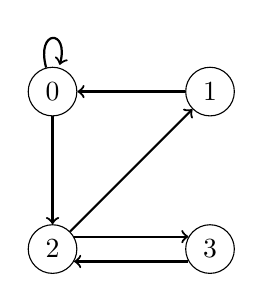
\begin{tikzpicture}
    \node[shape=circle,draw=black] (A) at (0,2) {0};
    \node[shape=circle,draw=black] (B) at (2,2) {1};
    \node[shape=circle,draw=black] (C) at (0,0) {2};
    \node[shape=circle,draw=black] (D) at (2,0) {3};
    \path  (A) edge [loop above, thick] (A);
    \path [->] (B) edge [thick] (A);  
    \path [->] (A) edge [thick] (C);  
    \path [->] (C) edge [thick] (B);  
    \path [->] (C.30) edge [thick] (D.150);  
    \path [->] (D.210) edge [thick] (C.-30);  
    \end{tikzpicture}
    \caption{The defined graph when $b = 4$. There are 4 nodes, each one corresponding to a value mod 4.}
    \label{fig:base_4_graph}
\end{figure}
There are 4 different nodes: one for each integer between 0 and 3. Because $4 = 2^2$, we are looking at the last 2 bits of each number. For example, a number congruent modulo to $0\Mod{4}$ has 00 as the 2 least significant bits, while a number congruent modulo to $2\Mod{4}$ has 10 as its 2 least significant bits. 
\subsection{Base 4 graph construction} \label{subsubsec:proofbase4graph}
Figure~\ref{fig:base_4_graph} shows the Base 4 Collatz Graph, and this subsection describes the construction of it. First, we will start with the even nodes, then the odd nodes:
\begin{itemize}
    \item Node 0 corresponds to the number ending with binary string ``00''. Removing the last 0 leaves either ``00'', looping to $0\Mod{4}$, or ``10'', changing it to $2\Mod{4}$.
    \item Node 2 corresponds to the number ending with binary string ``10''. Removing the last 0 leaves either ``01'', changing it to $1\Mod{4}$, or ``11'', changing it to $3\Mod{4}$.
\end{itemize}
Hence the even nodes and transitions from them are all correct. Now, the odd nodes:
\begin{itemize}
    \item Node 1 corresponds to the number ending with binary string ``01''. Multiplying this by 3 and adding 1 results in the binary number ending in ``$y_200$'', where $y_2$ is an unknown bit. Even though we don't know $y_2$, the number is still $0\Mod{4}$.
    \item Node 3 corresponds to the number ending with binary string ``11''. Multiplying this by 3 and adding 1 results in the binary number ending in ``$y_3y_210$'', which is still $2\Mod{4}$.
\end{itemize}
\subsection{Base 4 variants} \label{subsubsec:base4variants}
We introduced the Base 4 case for nodes because we can prove that we need to visit all of the nodes in this graph. This is equivalent to saying that each of the Collatz Variants, $\ColMod{N}{A}{4}$ terminates for nonempty $A \subseteq \{0,1,2,3\}$, and for any input number $N$. 
\begin{theorem}
Algorithm 4 terminates for nonempty $A \subseteq \{0,1,2,3\}$.
\end{theorem}
\begin{proof}
We will start with proving that $\ColMod{N}{2}{4}$ will terminate for any input number $N$, because the 2 node is central to the Base 4 graph.\par
\begin{lemma}
\label{lem:collatzSubTwoModFour}
$\ColMod{N}{2}{4}$ terminates for any $N$.
\end{lemma} 
\begin{proof}
We use the graph to help in this proof. An equivalent question is this: Can we show that node 2 must be visited for all input numbers? To show that this is the case, we have to show that all other nodes must visit node 2. 
\begin{itemize}
    \item 2: If the input number is this, we are already done.
    \item 3: This must, by definition, transition after the $3x+1$ mapping has been applied in one step.
    \item 1 and 0: 1 must transition to 0 after applying the $3x+1$ mapping once. For 0, use Lemma~\ref{lem:zeroCycle}(the ``0 cycle'' lemma) for $b = 4$, and the number will eventually transition to the 2 node.
\end{itemize}
Since all other nodes must visit node 2, it means that for all $N$, $\ColMod{N}{2}{4}$ terminates.
\end{proof} \par

\begin{lemma}
\label{lem:collatzSubOneModFour}
$\ColMod{N}{1}{4}$ terminates for any $N$.
\end{lemma}
\begin{proof}
We use Lemma~\ref{lem:collatzSubTwoModFour} to show that we need to visit node 2, and Lemma~\ref{lem:oneConsumption} to show that the cycle between nodes 2 and 3 cannot continue indefinitely, so node 2 must eventually transition to 1, proving termination of this variant.
\end{proof}
\begin{lemma}
\label{lem:collatzSubZeroModFour}
$\ColMod{N}{0}{4}$ terminates for any $N$.
\end{lemma}
\begin{proof}
Given Lemma~\ref{lem:collatzSubOneModFour}, we know we must visit node 1, and given Lemma~\ref{lem:numOutEdges}, an odd node can only have one outgoing edge, so it must transition to node 0.
\end{proof}
\begin{lemma}
\label{lem:collatzSubThreeModFour}
$\ColMod{N}{3}{4}$ terminates for any $N$.
\end{lemma}
\begin{proof}
Given Lemma~\ref{lem:EvenDom}, the $2 \rightarrow 1 \rightarrow 0 \rightarrow 2$ cycle cannot continue forever because if we assume that the 0 node never self-cycles, $2^2 > 3^1$. The 0 self-cycle makes even nodes dominate in number. So either $\ColMod{N}{3}{4}$ terminates by eventually becoming 1, or the cycle is broken... the only other node to visit is 3, also causing $\ColMod{N}{3}{4}$ to terminate.
\end{proof}
Since all of these lemmas hold, it follows that any singleton set from $A \subseteq \{0,1,2,3\}$ causes $\ColMod{N}{A}{4}$ to terminate. Also, by definition of Algorithm~\ref{alg:ColSP}, any larger size sets for $A$ also terminate as larger set sizes add more termination conditions.
\end{proof}
\section{Base 8 Graph and Variants} \label{subsec:base8graphsubpblms}
We showed that, using the Base 4 graph, $\ColMod{N}{A}{4}$ terminates for any nonempty base set $A$ and input number $N$. We decided to see what would happen if we expanded to $k = 3$ bits. We ran into a problem, and could not prove all variants of $\ColMod{N}{A}{8}$. This will motivate further computation undertaken in chapter~\ref{sec:subhrdnspred}, as we try to determine how hard figuring out these variants are. \par
Figure~\ref{fig:base_8_graph} shows the base 8 graph.
\begin{figure}
    \centering
    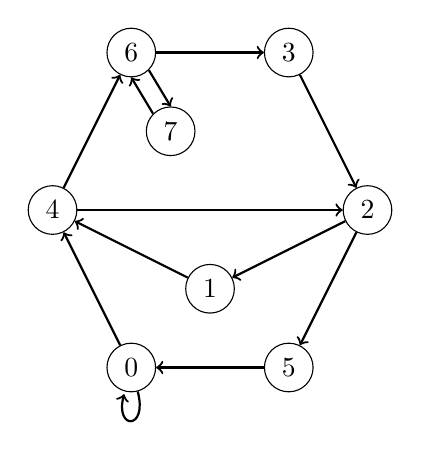
\begin{tikzpicture}
    \node[shape=circle,draw=black] (A) at (1,0) {0};
    \node[shape=circle,draw=black] (B) at (2,1) {1};
    \node[shape=circle,draw=black] (C) at (4,2) {2};
    \node[shape=circle,draw=black] (D) at (3,4) {3};
    \node[shape=circle,draw=black] (E) at (0,2) {4};
    \node[shape=circle,draw=black] (F) at (3,0) {5};
    \node[shape=circle,draw=black] (G) at (1,4) {6};
    \node[shape=circle,draw=black] (H) at (1.5,3) {7};
    \path  (A) edge [loop below, thick] (A);
    \path [->] (A) edge [thick] (E);  
    \path [->] (B) edge [thick] (E);  
    \path [->] (C) edge [thick] (B);  
    \path [->] (C) edge [thick] (F);  
    \path [->] (D) edge [thick] (C);  
    \path [->] (E) edge [thick] (C);  
    \path [->] (E) edge [thick] (G);  
    \path [->] (F) edge [thick] (A);  
    \path [->] (G) edge [thick] (D);  
    \path [->] (G.-45) edge [thick] (H.90);  
    \path [->] (H.135) edge [thick] (G.-90);  
    \end{tikzpicture}
    \caption{The defined graph when $b = 8$. There are 8 nodes, each one corresponding to a value mod 8.}
    \label{fig:base_8_graph}
\end{figure}
There are 8 different nodes, since $8 = 2^3$, and we are looking at the last 3 bits of each number. 
\subsection{Base 8 graph construction} \label{subsubsec:base8proof}
Like the base 4 graph, let us show how to construct the base 8 graph. Like in the base 4 case, let us examine the even nodes first. In this case, there are four different nodes: 0, 2, 4, and 6. Using Lemma~\ref{lem:numOutEdges}, each vertex has two different transitions, depending on what the next bit to the left of the 3 bits after removing the least significant 0. 
\begin{itemize}
    \item Node 0 corresponds to the binary string ``000''. Removing the last 0 leaves either ``000'', looping to $0\Mod{8}$, or ``100'', changing it to $4\Mod{8}$.
    \item Node 2 corresponds to the binary string ``010''. Removing the last 0 leaves either ``001'', changing it to $1\Mod{8}$, or ``101'', changing it to $5\Mod{8}$.
    \item Node 4 corresponds to the binary string ``100''. Removing the last 0 leaves either ``010'', changing it to $2\Mod{8}$, or ``110'', changing it to $6\Mod{8}$.
    \item Node 6 corresponds to the binary string ``110''. Removing the last 0 leaves either ``011'', changing it to $3\Mod{8}$, or ``111'', changing it to $7\Mod{8}$.
\end{itemize}
Hence the even nodes and transitions from them are all correct. Now, the odd nodes. Let $y_3$ and $y_4$ be unknown bits.
\begin{itemize}
    \item Node 1 corresponds to the binary string ``001''. Multiplying this by 3 and adding 1 results in the string ``100'', or $4\Mod{8}$.
    \item Node 3 corresponds to the binary string ``011''. Multiplying this by 3 and adding 1 results in the string ``$y_3010$'', which is $2\Mod{8}$.
    \item Node 5 corresponds to the binary string ``101''. Multiplying this by 3 and adding 1 results in the string ``$y_4y_3000$'', which is $0\Mod{8}$.
    \item Node 7 corresponds to the binary string ``111''. Multiplying this by 3 and adding 1 results in the string ``$y_4y_3110$'', which is $6\Mod{8}$.
\end{itemize}
So all of these transitions are correct as well, and our base 8 graph is correct.
\end{proof}
%CONTINUE WORK FROM HERE. TURN THIS INTO THE VARIANT VERSION.
\subsection{Base 8 variants} \label{subsubsec:base8subprob}
As for which nodes we are forced to visit during the computation of a $3x+1$ sequence, we can conditionally prove needing to visit nodes 0, 2, 3, 4, and 6, but we don't have proofs for 1, 5, and 7. Here are how we know we must visit the 5 nodes we know:


\begin{itemize}
    \item \textbf{Node 0}: Needs to transition from $5\Mod{8}$. We can't totally prove this yet unless we prove the need for $5\Mod{8}$.
    \item \textbf{Node 2}: We can get to $2\Mod{8}$ in two different ways: Either from $3\Mod{8}$, which is needed, or directly from $4\Mod{8}$. So $2 \Mod{8}$ is definitely needed. 
    \item \textbf{Node 3}: Given Lemma~\ref{lem:oneConsumption}, a $6 \rightarrow 7 \rightarrow 6$ cycle cannot continue forever. Hence, $6\Mod{8}$ must transition to $3\Mod{8}$ eventually.
    \item \textbf{Node 4}: We know that we need $2\Mod{8}$ already. Both possible paths come from that node: Either we visit $1\Mod{8}$ then transition to $4\Mod{8}$, or we visit $5\Mod{8}$ then $0\Mod{8}$. From Lemma~\ref{lem:zeroCycle}, the 0 cycle cannot continue forever, so the number will eventually be $4\Mod{8}$.
     \marginnote{I do NOT like this explanation for Node 6. Needs to be retooled.}
    \item \textbf{Node 6}: If a $3x+1$ sequence never visited $6\Mod{8}$, it would be forced into one of two cycles: $4 \rightarrow 2 \rightarrow 1$ or $4 \rightarrow 2 \rightarrow 5 \rightarrow 0 \rightarrow \ldots \rightarrow 4$, where $\ldots$ is 0 or more repetitions of the 0 node being revisited. Both of these cycles cause the number to decrease in size, especially the second one, because both are dividing by at least 4 compared to the multiplication by 3. If all numbers followed these cycles, we would never have any numbers grow large in size, but we have several counterexamples showing that numbers do grow quite large, so hence, $6\Mod{8}$ must be visited as well.
   
\end{itemize}
1, 5, and $7\Mod{8}$ do not have proofs. All three numbers come from a even node, meaning each of these has two choices. Hence, we've run some computational experiments to try and better understand the difficulty of calculating these numbers as standalone nodes, and also as pairs. 
\subsection{Cycle analysis} \label{subsubsec:cycleanalysis}
In this section we provide a bit analysis of cycles in the base 8 graph, and show how several of these are equivalent to showing certain nodes are needed to be visited, and hence, how they tie to certain Collatz Variants.
\begin{itemize}
    \item The 0 self-cycle cannot continue forever, as per Lemma~\ref{lem:zeroCycle}.
    \item The $6 \rightarrow 7 \rightarrow 6$ cycle cannot continue forever as per Lemma~\ref{lem:oneConsumption}.
    \item The $4 \rightarrow 2 \rightarrow 1 \rightarrow 4$ cycle: Left blank, see margin note. \marginnote{Working on the $4 \rightarrow 2 \rightarrow 1 \rightarrow 4$ cycle, don't have a proof yet, but I think it's provable.}
    \item $4 \rightarrow 2 \rightarrow 5 \rightarrow 0 \rightarrow 4$ cycle: The proof for avoiding this cycle stems directly from the proof for node $6$ being required. This cycle can also include visits to node $1$ as well.
    \item $4 \rightarrow 6 \rightarrow 3 \rightarrow 2 \rightarrow 1 \rightarrow 4$ cycle: We don't have a proof for this cycle. Proving this doesn't hold and we have to break it is equivalent to proving that 5 and 7$\Mod{8}$ both cannot be avoided, a proof we explore in section~\ref{sec:subhrdnspred}. NOTE: If we allow visits to 7 in the cycle as well, then this proof would be equivalent to avoiding just $5 \Mod{8}$.
    \item $4 \rightarrow 6 \rightarrow 3 \rightarrow 2 \rightarrow 5 \rightarrow 0 \rightarrow 4$ cycle: There are three different variations to showing this cycle cannot continue forever, all of them unproven, and all of them lead to interesting questions.
    \begin{itemize}
        \item Allowing 7 but avoiding 1: This cycle is equivalent to showing why we need 1$\Mod{8}$. This proof might be challenging, because we'd have two conflicting cycles: one which causes the number to grow by 3/2 every time, and another one to divide by 2 every time. Our findings in section~\ref{sec:subhrdnspred} suggest this may be a cycle that grows in difficulty to find a proof as the numbers get larger.
        \item Allowing 1 but avoiding 7: This cycle is equivalent to the proof of why we need 7$\Mod{8}$. 
        \item Avoiding both 1 AND 7: This would be equivalent to the 1 and 7$\Mod{8}$ avoidance combination. We explore this combination in section~\ref{sec:subhrdnspred}.
    \end{itemize}
\end{itemize}